\section{Contenedorización}
%TODO actualizar con este tuto https://docker-curriculum.com/

\subsection{Contenedores versus VMs}

\begin{frame}{Contenedorización}
 \begin{itemize}
  \item El uso de contenedores Linux para implementar aplicaciones se denomina \textbf{contenedorización}. 
  \item Los contenedores no son nuevos, pero su uso para implementar aplicaciones fácilmente sí lo es.
  \item \textbf{Contenedor} $\longrightarrow$ ejemplar en tiempo de ejecución de una imagen (cargada en memoria).
  \item \textbf{Imagen} $\longrightarrow$ paquete ejecutable que incluye todo lo necesario para ejecutar una aplicación: código, entorno de ejecución, bibliotecas, variables de entorno y archivos de configuración.
 \end{itemize}
 \begin{alertblock}{Docker}
  Plataforma para desarrolladores y administradores de sistemas para desarrollar, implementar y ejecutar aplicaciones con contenedores. Permite separar las aplicaciones de la infraestructura para desplegar software rápidamente.
 \end{alertblock}
\end{frame}

\begin{frame}{Contenedores versus VMs}
 \begin{itemize}
  \item Un contenedor se ejecuta nativamente en Linux y comparte el kernel de la máquina host con otros contenedores. 
  \item Un contenedor se ejecuta como cualquier otro proceso, no teniendo más memoria que otro ejecutable (lightweight).
  \item Una máquina virtual (VM) ejecuta un sistema operativo ``invitado'' completo con acceso virtual a recursos de host a través de un hipervisor. 
  \item En general, las VM proporcionan un entorno con más recursos de los que la mayoría de las aplicaciones necesitan. 
 \end{itemize}
 \begin{center}
  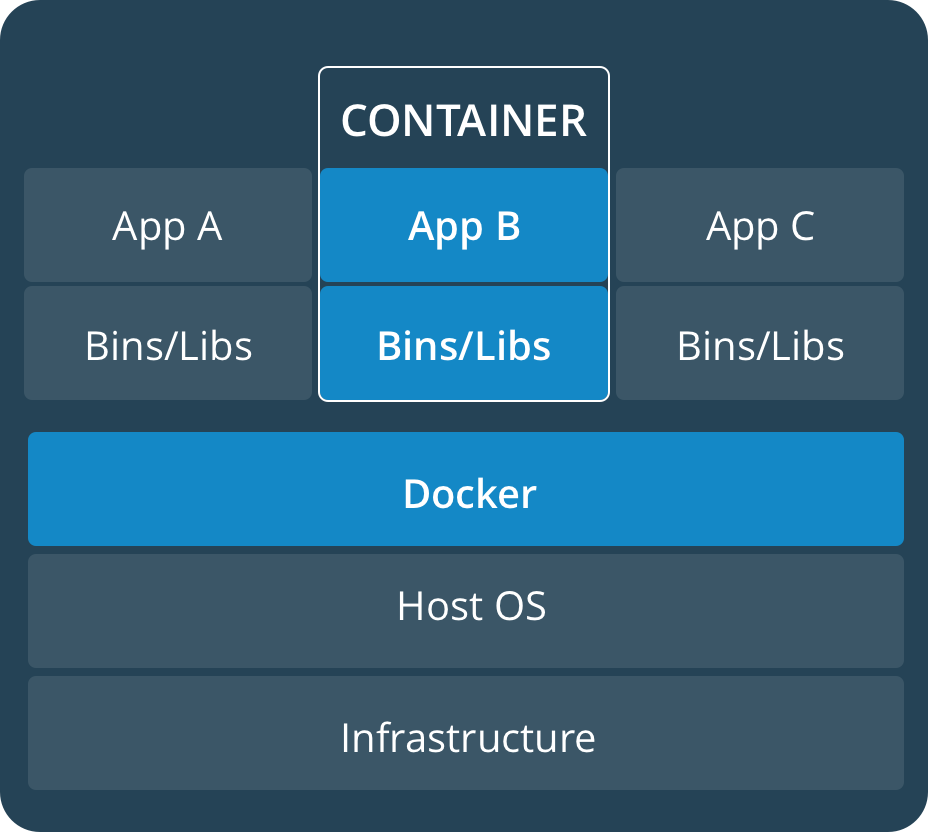
\includegraphics[height=3cm]{img/contenedor.png}~~~
  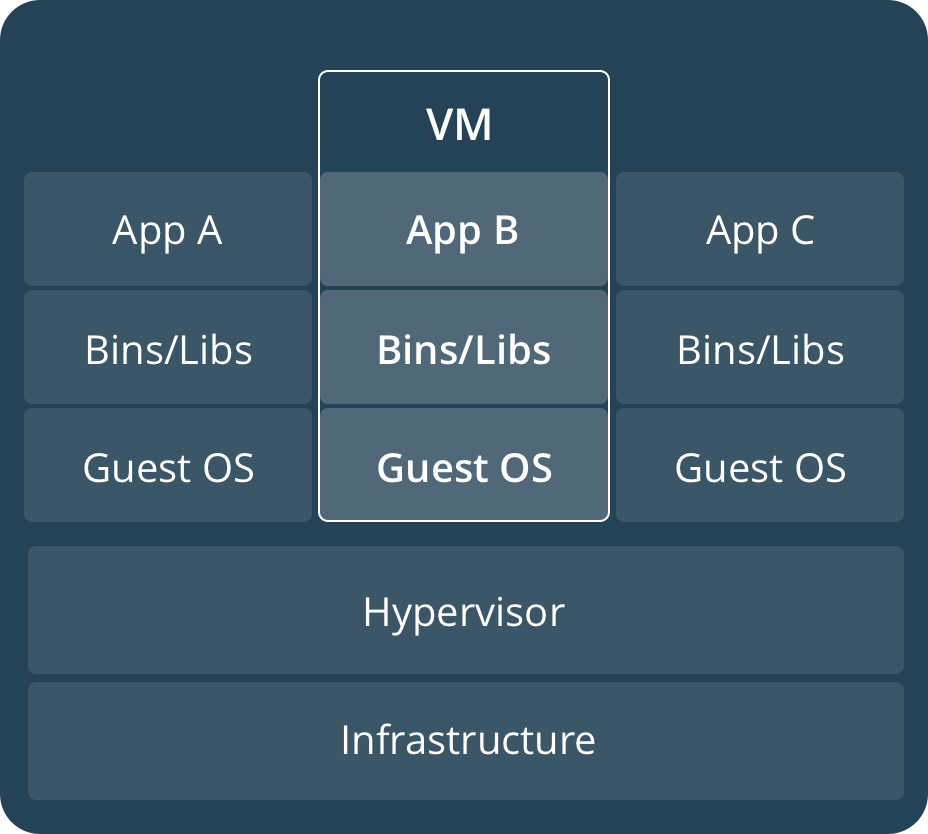
\includegraphics[height=3cm]{img/VM.png}
 \end{center}
\end{frame}

\subsection{Get started}

\begin{frame}[fragile,allowframebreaks]{Docker installation}
\begin{enumerate}
 \item Set up the repository:
\begin{lstlisting}[language=shell]
$ sudo apt-get update # Update the package index
$ sudo apt-get install ca-certificates curl gnupg lsb-release # Install packages to allow apt to use a repository over HTTP
$  curl -fsSL https://download.docker.com/linux/ubuntu/gpg | sudo gpg --dearmor -o /usr/share/keyrings/docker-archive-keyring.gpg  # Add Docker's official GPG key
$ echo "deb [arch=$(dpkg --print-architecture) signed-by=/usr/share/keyrings/docker-archive-keyring.gpg] https://download.docker.com/linux/ubuntu $(lsb_release -cs) stable" | sudo tee /etc/apt/sources.list.d/docker.list > /dev/null # Use the following command to set up the stable repository
\end{lstlisting}
 \framebreak
 \item Install Docker CE:
\begin{lstlisting}[language=shell]
$ sudo apt-get update # Update the package index
$ sudo apt-get install apt-get install docker-ce docker-ce-cli containerd.io # Install the latest version of Docker CE
$ sudo docker run hello-world # Verify that Docker CE is installed correctly by running the hello-world image.
...
Hello from Docker!
This message shows that your installation appears to be working correctly.
...
\end{lstlisting}

 \item Post-installation
  \begin{itemize}
   \item Manage Docker as a non-root user:
\begin{lstlisting}[language=shell]
$ sudo groupadd docker # Create the docker group
$ sudo usermod -aG docker $USER # Add your user to the docker group. Log out and log back in so that your group membership is re-evaluated or run 'newgrp docker' to activate the changes to groups
$ docker run hello-world # Verify that you can run docker commands without sudo
\end{lstlisting}
  \end{itemize}
\end{enumerate}
\end{frame}

% \begin{frame}[fragile]{BusyBox}
%  \begin{itemize}
%   \item Fetch the \textbf{busybox} image from the \textbf{Docker registry}:
% \begin{lstlisting}[language=shell]
% $ docker pull busybox
% \end{lstlisting}
  
%   \item You can use the \texttt{docker images} command to see a list of all images on your system:
% \begin{lstlisting}[language=shell]
% $ docker images
% \end{lstlisting}

%   \item Run a Docker container based on this image:
% \begin{lstlisting}[language=shell]
% $ docker run busybox
% $
% $ docker run busybox echo "hello from busybox"
% hello from busybox
% \end{lstlisting}
  
%   \item \texttt{docker ps} command shows you all containers that are currently running.
% \begin{lstlisting}[language=shell]
% $ docker ps
% CONTAINER ID        IMAGE               COMMAND             CREATED             STATUS              PORTS               NAMES
% $ docker ps -a
% ...
% \end{lstlisting}
%  \end{itemize}
% \end{frame}

\begin{frame}[fragile]{Basic commands}
 \begin{itemize}
  \item List Docker CLI commands:
\begin{lstlisting}[language=shell]
$ docker
$ docker container --help
\end{lstlisting}

  \item Display Docker version and info:
\begin{lstlisting}[language=shell]
$ docker --version
$ docker version
$ docker info
\end{lstlisting}

  \item Execute Docker images:
\begin{lstlisting}[language=shell]
$ docker run hello-world
$ docker run -it <image> sh # -it attaches us to an interactive tty in the container
\end{lstlisting}

  \item List Docker images/networks/containers:
\begin{lstlisting}[language=shell]
$ docker image ls
$ docker network ls
$ docker container ls        # containers running
$ docker container ls --all  # all
$ docker container ls -a -q  # all in quiet mode
$ docker ps
\end{lstlisting}
 \end{itemize}
\end{frame}

\subsection{Define a container}

\begin{frame}[fragile]{Sample application}
 \begin{itemize}
  \item Create a simple Python application using the Flask framework:
\begin{lstlisting}[language=shell]
$ cd /path/to/app
$ pip3 install Flask
$ pip3 freeze | grep Flask >> requirements.txt
$ touch app.py  
\end{lstlisting}

  \item Enter the following code into the \texttt{app.py} file:
\begin{lstlisting}[language=python]
from flask import Flask
app = Flask(__name__)

@app.route('/')
def hello_world():
    return 'Hello, Docker!'
\end{lstlisting}
  
  \item Test the application:
\begin{lstlisting}[language=shell]
$ pwd
/path/to/app
$ python3 -m flask run
\end{lstlisting}
  
  \item Open a browser and navigate to \texttt{http://localhost:5000}. Switch back to the terminal where the server is running and you should see the requests in the server logs.
 \end{itemize}
\end{frame}


\begin{frame}[fragile]{Create a Dockerfile}
\begin{itemize}
  \item \textit{Dockerfile} defines what goes on in the environment inside your container:
\begin{lstlisting}[language=syntax]
FROM python:3.8-slim-buster # Docker images inherit from other base images

WORKDIR /app # default location for all subsequent commands

COPY requirements.txt requirements.txt # copy files into the image
RUN pip3 install -r requirements.txt # execute the command
#RUN pip3 install Flask # Uncomment on Windows and Mac and comment the above lines

COPY . . # Takes all the files located in the current directory and copies them into the image

CMD [ "python3", "-m" , "flask", "run", "--host=0.0.0.0"] # Command to run when the image is executed inside a container
\end{lstlisting}

 \item The Python application directory (\texttt{/path/to/app}) structure would now look like:
\begin{lstlisting}
app
|____ app.py
|____ requirements.txt
|____ Dockerfile
\end{lstlisting}
\end{itemize}
\end{frame}

\begin{frame}[fragile]{Build and run the app}
\begin{itemize}
 \item Build the app:
\begin{lstlisting}[language=shell]
$ pwd
/path/to/app
$ docker build --tag sample-app .
...
$ docker images
...
\end{lstlisting}
 \item Run the app:
\begin{lstlisting}[language=shell]
$ docker run --publish 5000:5000 sample-app
\end{lstlisting}

 \item In a new terminal:
\begin{lstlisting}[language=shell]
$ curl localhost:5000
Hello, Docker!
\end{lstlisting}

 \item Run the app in the background, in detached mode:
\begin{lstlisting}[language=shell]
$ docker run -d -p 5000:5000 sample-app
$ docker ps
$ docker stop CONTAINER_ID
$ docker ps
\end{lstlisting}
\end{itemize}
\end{frame}

\subsection{Rocker}
\begin{frame}[fragile]{Rocker}

 \begin{alertblock}{Rocker}
  Herramienta que permite ejecutar imágenes de Docker con soporte local, por ejemplo soporte de nvidia. Dando la posibilidad de abrir interfaces gráficas en el equipo host. 
  
  \url{https://github.com/osrf/rocker}
 \end{alertblock}

\begin{itemize}
    \item Installation:
\begin{lstlisting}[language=shell]
$ pip install rocker
\end{lstlisting}

    \item Extensions:
    \begin{itemize}
        \item x11 -- Enable the use of X11 inside the container via the host X instance.
        \item nvidia -- Enable NVIDIA graphics cards for rendering
        \item cuda -- Enable NVIDIA CUDA in the container
        \item user -- Create a user inside the container with the same settings as the host and run commands inside the container as that user.
        \item home -- Mount the user's home directory into the container
        \item pulse -- Mount pulse audio into the container
        \item ssh -- Pass through ssh access to the container.
    \end{itemize}
\end{itemize}
    
\end{frame}

\subsection{Docker Hub}
\begin{frame}[fragile]{Docker Hub}
\begin{alertblock}{Docker Hub}
    Repositorio de imágenes docker.
  
  \url{https://hub.docker.com/}
 \end{alertblock}
 
\begin{itemize}
    \item Download an image:
\begin{lstlisting}[language=shell]
$ docker pull <name of the image>
\end{lstlisting}
    
\end{itemize}
    
\end{frame}

